\documentclass[a4j]{jarticle}
\usepackage[dvipdfmx]{graphicx,color}
\usepackage{verbatim}
\usepackage{ascmac}
\usepackage{url}
\usepackage{listings,jlistings}
\usepackage{color}
%\setlength{\marginparwidth}{20mm}%% 傍注欄の横幅の設定

\input{/home/ryousuke/listings_temp.tex}

\title{情報科学プロジェクト実験レポート課題}
\author{S142063 佐藤涼亮}

\begin{document}
\maketitle
\centerline{\LARGE \underline{Webアプリケーション}}
\section{課題の内容}
{\large \underline{Webアプリケーションの作成}}
\subsection{要点}
\begin{enumerate}
\item ユーザのログインとクッキーの管理
\item ユーザごとの最高点をデータベースで管理
\item ユーザごとの最高点のうちベスト10をゲーム画面の横に表示
\end{enumerate}
\section{プログラムの説明}
ログイン画面とゲーム画面(アプリ画面)を作成し、それぞれのに対応した処理を行う。
ログイン画面には、ユーザー名とパスワードの入力欄を設け、
ログインに必要な情報の入力を求め、ログインを行う。
ログインされたアカウント情報をデータベースで検索し、
新しいアカウント情報なら登録、
既存のアカウント情報なら更新し、
cookieを設定してゲーム画面に移行する。
ゲーム画面では、ゲームに加え、既存のアカウントでの得点ランキングや
ユーザーが今回獲得した得点を表示している。
獲得した得点は、猫を倒すごとに加算されるようになっていて、
ゲームオーバになると同時に、データベースへその記録が格納されるようになっている。
cookieの有効期限は登録、更新した時からセッションが終了するまでとする。
\newpage
入力されたユーザー情報は、獲得した最高得点やcookieとともにデータベースに格納される。
データベースのテーブル、スキーマは以下の通りである。\\*
\begin{screen}
\begin{verbatim}
sqlite> .table
accountScore
sqlite> .schema
CREATE TABLE accountScore(
user text not null,
pass text not null,
score int,
cookie text
);
sqlite>
\end{verbatim}
\end{screen}

\subsection{目的}
Webアプリケーションの作成

\subsection{方法}
JavaScript,HTML,CGI,C++を用いる

\subsection{結果}

\begin{center}
ログイン画面\\*
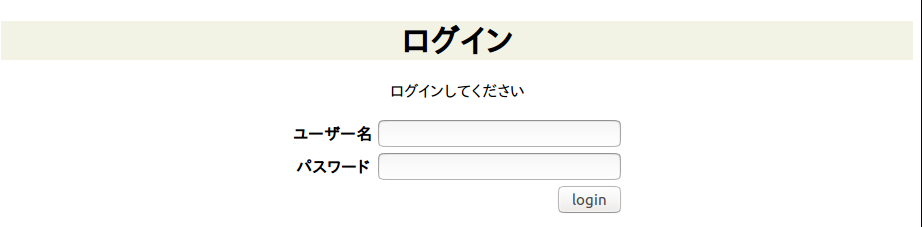
\includegraphics[width=\textwidth]{result/result1.png}\\*

{\LARGE↓}

ゲーム画面\\*
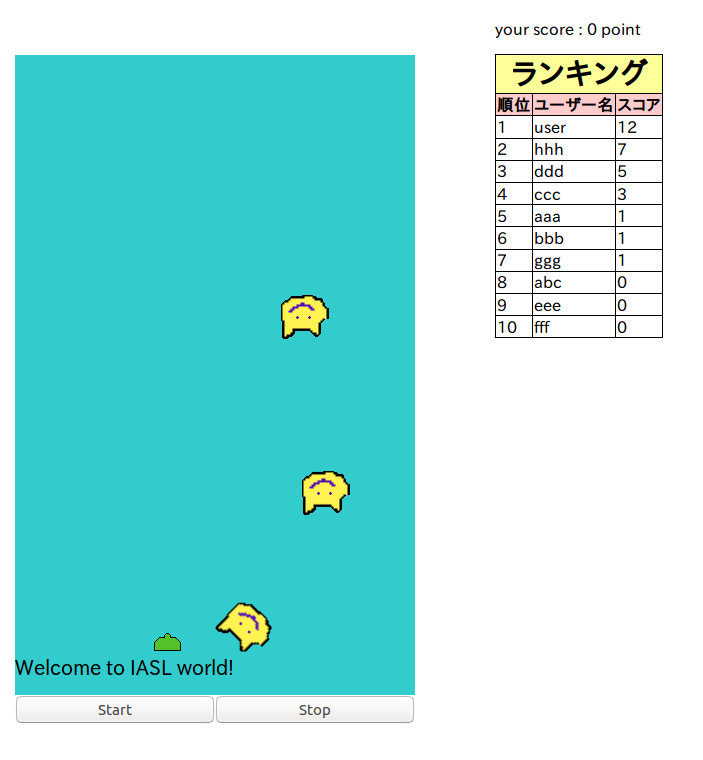
\includegraphics[width=\textwidth]{result/result2.png}\\*
\end{center}

\newpage
\subsection{考察}
以下が、結果で見られるユーザー情報やランキングである。\\*
\begin{screen}
\begin{verbatim}
sqlite> select * from accountScore order by score desc;
user|pass|12|82582066
hhh|hhh|7|58150040
ddd|ddd|5|58086813
ccc|ccc|3|58051599
aaa|aaa|1|97125618
bbb|bbb|1|58035592
ggg|ggg|1|58138835
abc|abc|0|97108010
eee|eee|0|58114825
fff|fff|0|58126030
iii|iii|0|58162845
sqlite> 
\end{verbatim}
\end{screen}\\

これらより、データの格納・更新は成功し、
Webアプリケーションを作成することができた。

\section{感想}
今回、今までの実験の内容を応用し、
簡単なWebアプリケーションを作成した。
時間がなく、レイアウトが拙くなり、デザインが悪くなってしまった。
HTML/CSSデザインを学んだが、経験が少ないこともあり、
装飾やレイアウトをどのように変え、どのようにデザインをすればいいのか、
まだわからないことだらけである。

順位表示は、タイ表示も考えたが、
10位以内にタイが多いとランキングも無駄に大きくなってしまうので、
ユーザー名の辞書順に表示するようにした。

\section{プログラム}
\lstinputlisting[caption=iasl.cpp]{iasl.cpp}
\lstinputlisting[caption=store.cpp]{store.cpp}
\lstinputlisting[caption=iasl\_html.js,language=javascript]{iasl\string_html.js}
\lstinputlisting[caption=iasl\_ja.js,language=javascript]{iasl\string_ja.js}

\end{document}
